\documentclass[a4paper, 10pt]{article}
% (1) Encoding, Fonts, and Layout
\usepackage[T1]{fontenc}
\usepackage{lmodern}
\usepackage[margin=1in]{geometry}


% (2) Common Packages
\usepackage{amsmath, amssymb, amsthm}
\usepackage{xcolor}
\usepackage{caption}
\usepackage{tikz}
\usepackage{pgfplots}
\pgfplotsset{compat=newest}
\usepackage{etoolbox}
\usepackage{tikz-3dplot}
\tdplotsetmaincoords{75}{120}
\usepackage[inline]{enumitem}
\usepackage{bookmark}
\usepackage{mathtools}
\usepackage{subcaption} % For subfigures
\usepackage[normalem]{ulem} % For better underline commands

% Micro-typography
\usepackage{microtype}

% Patching pgfplots warning
\makeatletter
\patchcmd{\pgfplots@applistXXpushback@smallbuf}{\pgfplots@error}{\pgfplots@warning}{}{}
\makeatother

% (3) tcolorbox and Theorem Libraries
\usepackage{tcolorbox}
\tcbuselibrary{theorems}

% (4) Define Colors
\definecolor{custom_green}{HTML}{a3be8c}
\definecolor{custom_red}{HTML}{dc322f}
\definecolor{custom_blue}{HTML}{268bd2}
\definecolor{custom_purple}{HTML}{b48ead}

\definecolor{base}{HTML}{eceff4}
\definecolor{gray1}{HTML}{e5e9f0}
\definecolor{gray2}{HTML}{d8dee9}
\definecolor{gray3}{HTML}{2e3440}
\pagecolor{base}

% (5) Custom tcolorbox Environments
\newtcolorbox{definitionbox}[1][]{
    title=\textbf{Definition} {#1},
    fonttitle=\bfseries\boldmath,
    arc=0mm,
    bottomtitle=0.5mm,
    boxrule=0mm,
    colbacktitle=gray2,
    colback=gray1,
    coltitle=gray3,
    coltext=gray3,
    left=2.5mm,
    leftrule=1mm,
    rightrule=1mm,
    right=3.5mm,
    toptitle=0.75mm,
    colframe=custom_red,
}

\newtcolorbox{proofbox}{
    title=\textbf{Proof},
    fonttitle=\bfseries\boldmath,
    arc=0mm,
    bottomtitle=0.5mm,
    boxrule=0mm,
    colbacktitle=gray2,
    colback=gray1,
    coltitle=gray3,
    left=2.5mm,
    leftrule=1mm,
    rightrule=1mm,
    right=3.5mm,
    toptitle=0.75mm,
    colframe=custom_blue,
    coltext=gray3,
}

\newtcolorbox{theorembox}[1][]{
    title=\textbf{Theorem} {#1},
    fonttitle=\bfseries\boldmath,
    arc=0mm,
    bottomtitle=0.5mm,
    boxrule=0mm,
    colbacktitle=gray2,
    colback=gray1,
    coltitle=gray3,
    left=2.5mm,
    leftrule=1mm,
    rightrule=1mm,
    right=3.5mm,
    toptitle=0.75mm,
    colframe=custom_green,
    coltext=gray3
}

\newtcolorbox{notebox}{
    title=\textbf{Note},
    fonttitle=\bfseries\boldmath,
    arc=0mm,
    bottomtitle=0.5mm,
    boxrule=0mm,
    colbacktitle=gray2,
    coltitle=gray3,
    left=2.5mm,
    leftrule=1mm,
    rightrule=1mm,
    right=3.5mm,
    toptitle=0.75mm,
    colframe=custom_blue,
    coltext=gray3
}

\newtcolorbox{examplebox}[1][]{
    title=\textbf{Example} {#1},
    fonttitle=\bfseries\boldmath,
    arc=0mm,
    bottomtitle=0.5mm,
    boxrule=0mm,
    colbacktitle=gray2,
    colback=gray1,
    coltitle=gray3,
    left=2.5mm,
    leftrule=1mm,
    rightrule=1mm,
    right=3.5mm,
    toptitle=0.75mm,
    colframe=gray3,
    fontupper=\footnotesize,
    coltext=gray3
}

% (6) Theorem Environments
\theoremstyle{definition}
\newtheorem{definition}{Definition}[section]
\newtheorem{example}[definition]{Example}

\theoremstyle{plain}
\newtheorem{theorem}[definition]{Theorem}

% (7) Hyperlinks
\usepackage{hyperref}
\hypersetup{
    colorlinks=true,    % Use colored text for links
    linkcolor=custom_red,      % Set link text color to red
    pdfborder={0 0 0}   % Remove the default box around links
}


% macros.tex
\newcommand{\intinf}{\int_0^{\infty}} % Integral from 0 to infinity
\newcommand{\diff}[2]{\frac{d#1}{d#2}} % Derivative


\title{
\textbf{MA2287: Complex Analysis} \\ 
}


\author{
  60\% Exam\\
  30\% Continuous Assessment (Homework) \\
  Robert Davidson
}   

 

\date{} % Empty date

\begin{document}

\maketitle
\pagebreak
\tableofcontents
\pagebreak


\section{Preliminary}
\subsection{The Complex Plane and the Four Quadrants}

\begin{minipage}{0.5\textwidth}
  The complex plane is a two-dimensional plane where the horizontal axis represents the real part and the vertical axis represents the imaginary part of a complex number. It is divided into four quadrants:
\end{minipage}
\begin{minipage}{0.5\textwidth}
  \begin{center}
    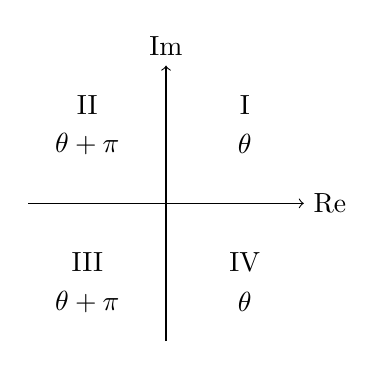
\begin{tikzpicture}[scale=1]
      % Draw axes
      \draw[->] (-1.75,0) -- (1.75,0) node[right] {\text{Re}};
      \draw[->] (0,-1.75) -- (0,1.75) node[above] {\text{Im}};


      % Label quadrants
      \node at (1,1.25) {I};
      \node at (-1,1.25) {II};
      \node at (-1,-0.75) {III};
      \node at (1,-0.75) {IV};

      \node at (1,0.75) {$\theta$};
      \node at (-1,0.75) {$\theta + \pi$};
      \node at (-1,-1.25) {$\theta + \pi$};
      \node at (1,-1.25) {$\theta$};
    \end{tikzpicture}
  \end{center}
\end{minipage}




\section{Foundations}
\subsection{Intro to Complex Numbers}
\noindent
\begin{minipage}{0.5\textwidth}
  Complex numbers can be written as the sum of a real and imaginary part:
  $$
    z = x + iy
  $$
  We denote the \textbf{complex conjugate} \((\overline{z})\) as:
  $$
    \overline{z} = x - iy
  $$
  Geometrically, $\overline{z}$ is the \textbf{reflection of z in the real axis}
\end{minipage}
\begin{minipage}{0.48\textwidth}
  \centering
  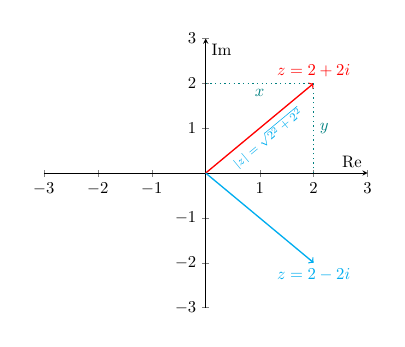
\begin{tikzpicture}[scale=0.6]
    \begin{axis}[
        axis lines = center,
        xlabel = {Re},
        ylabel = {Im},
        xmin = -3, xmax = 3,
        ymin = -3, ymax = 3,
        xtick = {-3,-2,...,3},
        ytick = {-3,-2,...,3},
      ]
      % Red arrow from (0,0) to (2,2)
      \addplot[->, thick, red]
      coordinates {(0,0) (2,2)}
      node[pos=1, above] {$z = 2 + 2i$}
      node[pos=0.5, sloped, below, cyan, font=\scriptsize] {$|z| = \sqrt{2^2+2^2}$};

      \addplot[->, thick, cyan]
      coordinates {(0,0) (2,-2)}
      node[pos=1, below] {$z =2  - 2i$};


      % Dotted vertical line (labeled y) from (2,0) to (2,2)
      \addplot[dotted, thick, teal]
      coordinates {(2,0) (2,2)}
      node[midway, right] {$y$};

      % Dotted horizontal line (labeled x) from (0,2) to (2,2)
      \addplot[dotted, thick, teal]
      coordinates {(0,2) (2,2)}
      node[midway, below] {$x$};

    \end{axis}
  \end{tikzpicture}
\end{minipage}



\noindent \\
With help from Pythagoras' we can now define the distance of $z$ from the origin (\textbf{modulus}), that is the length of the vector pointing to $z$.
$$|z|^2 = x^2 + y^2 \Rightarrow |z| = \sqrt{x^2 + y^2}$$
We notice that:
\begin{align*}
  z\overline{z} & = (x + iy)(x - iy)           \\
                & = x^2 - ixy + ixy - (iy)(iy) \\
                & = x^2 - (i)^2(y^2)           \\
                & = x^2 - (-1)(y^2)            \\
                & = x^2 + y^2                  \\
                & = |z|^2
\end{align*}
Thus, we have the distance of z from the origin as: $|z| = \sqrt{z\overline{z}} = \sqrt{x^2 + y^2}$
We refer to this as the \textbf{modulus} of $z$ or the \textbf{absolute value} of $z$. \\
Letting $z = x + iy$ and $w = u+iv$, we see:
$$|z -w| = \sqrt{(x-u)^2 + (y-z^2)^2}$$
That is, $|z-w|$ is the distance between $z$ and $w$ in the complex plane.


\subsection{Polar Form}

\begin{minipage}{0.48\textwidth}
  Letting \(r = |z| = \sqrt{x^2 + y^2}\), we can define \(x\) and \(y\) as:
  \begin{align*}
    \cos(\theta) & = \frac{x}{r} \quad\Rightarrow\quad x = r\cos\theta, \\
    \sin(\theta) & = \frac{y}{r} \quad\Rightarrow\quad y = r\sin\theta.
  \end{align*}

\end{minipage}\hfill
\begin{minipage}{0.48\textwidth}
  \centering
  \begin{tikzpicture}[scale=0.7]
    \begin{axis}[
        axis lines = center,
        xlabel = {Re},
        ylabel = {Im},
        xmin = -3, xmax = 3,
        ymin = -3, ymax = 3,
        xtick=\empty,
        ytick=\empty,
        clip=false,
      ]
      % Draw the blue vector from (0,0) to (2,2)
      \addplot[->, thick, blue]
      coordinates {(0,0) (2,2)}
      node[midway, sloped, above, blue] {$r = |z|$}
      node[pos=1, right] {$z = r(\cos\theta + i\sin\theta)$};

      % Draw an arc from the positive Re axis to the vector to represent theta.
      \draw[blue, thick] (axis cs:1,0) arc (0:45:1);

      % Label the theta angle near the arc.
      \node[blue] at (axis cs:0.5,0.25) {$\theta$};

      % Dotted lines representing the x and y components.
      \addplot[dotted, thick, gray]
      coordinates {(2,0) (2,2)}
      node[midway, right] {$y$};
      \addplot[dotted, thick, gray]
      coordinates {(0,2) (2,2)}
      node[midway, above] {$x$};

    \end{axis}
  \end{tikzpicture}
\end{minipage}
Now:
\begin{align*}
  z & = x + iy                       \\
    & = r\cos\theta + ir\sin\theta   \\
    & = r(\cos\theta + i\sin\theta).
\end{align*}
\noindent To find $\theta$ we usualy calculate $\tan^{-1}(y/x)$ and add/subtract $\pi$, when appropriate. Recalling $\tan^{-1}(y/x) \in (-\pi/2, \pi/2)$.
We denote $\theta$ as  as the \textbf{argument of z}, denoted as $\arg(z)$. Geometrically $\arg(z)$ represent the angle $z$ makes with the positive real axis
Thus, the pair (r, arg(z)) is called the \textbf{polar coordinates of z}.
We introduce the idea that $\arg(z)$ is a version of Arg$(z)$ that can take multiple values outside of Arg$(z)$'s bounds, ($-\pi, \pi$), more precisely:
$$\arg(z) = \text{Arg}(z) + 2 n \pi, \quad n \in \mathbb{Z}$$

\begin{examplebox}{Find $\text{Arg}(i)$ and $\arg(i)$}{}
  Since $i = 0 + 1i$, we have $x = 0$ and $y = 1$.

  Using $\tan^{-1}\left(\frac{y}{x}\right) \Rightarrow \arg(z) = \tan^{-1}\left(\frac{1}{0}\right) = \frac{\pi}{2}$


  Therefore:

  $$ \text{Arg}(i) = \frac{\pi}{2} \quad \text{and} \quad \arg(i) = \frac{\pi}{2} + 2n\pi, \quad n \in \mathbb{Z} $$
\end{examplebox}

\subsection{De Moivre's Theorem}
\textbf{Theorem:} Let $z_1,z_2 \in \mathbb{C}$, be nonzero numbers
$$z_1 = r_1(\cos\theta_1 + i\sin\theta_1) \quad \text{and} \quad z_2 = r_2(\cos\theta_2 + i\sin\theta_2)$$
Then:
\begin{align*}
  z_1z_2 & = r_1r_2[(cos\theta_1\cos\theta_2  + \sin\theta_1\sin\theta_2) + i(\sin\theta_1\cos\theta_2 + \cos\theta_1\sin\theta_2)] \\
         & = r_1r_2[\cos(\theta_1 + \theta_2) + i\sin(\theta_1 + \theta_2)]
\end{align*}
Thus, we have:
\begin{align*}
  |z_1z_2|     & = |z_1||z_2|            \\
  \arg(z_1z_2) & = \arg(z_1) + \arg(z_2)
\end{align*}

\begin{theorembox}[Corollary: De Moivre's Theorem]
  Let $n \in \mathbb{Z}$, and $z = |z|(\cos\theta + i\sin\theta)$, then:
  $$z^n = |z|^n = [\cos(n\theta) + i\sin(n\theta)]$$
\end{theorembox}

\subsection{Roots of Unity}
\textbf{Roots of unity are solutions to} $z^n = 1$, where $z$ is a complex number on the unit circle.\\
\textbf{Eulers formula} states that $e^{i\alpha} = \cos\alpha + i\sin\alpha$. \\
Given $z = x+ iy$, then:
$$z = r(\cos\theta + i\sin\theta) = re^{i\theta}$$
Since $z$ lies on the unit circle, we know $R =1$, thus we have
$$z = e^{i\theta}$$
Also, we can rewrite $1$ as:
\begin{align*}
  1 & = 1 + 0i = \cos(0) + i\sin(0)                                                                                                             \\
    & = \cos(2\pi) + i\sin(2\pi) = \cos(2\pi k) + i\sin(2\pi k) \quad (\text{Periodic with} 2\pi \; \text{k multiples don't change the result}) \\
    & = e^{i2\pi k} \quad \text{where} \; k \in \mathbb{Z} \quad (\text{By Eulers Formula})
\end{align*}
So we have, $z^n = e^{n(i \theta)}$:
\begin{align*}
  e^{in\theta} & = e^{i2\pi k}      \\
  in\theta     & = i 2\pi k         \\\
  n\theta      & = 2\pi k           \\
  \theta       & = \frac{2\pi k}{n}
\end{align*}
So $\theta$ is the angle corresponding to the $n$-th roots of unity. Using eulers formula again, the solutions are given as:
$$z^k = e^{i\theta} = e^{i(\frac{2\pi k}{n})} = \cos\left(\frac{2\pi k}{n}\right) + i \sin\left(\frac{2\pi k}{n}\right)$$

\begin{proofbox}[Conjugate Roots Theorem]

  Let $p(z) = a_nz^n + a_{n-1}z^{n-1} + \cdots + a_1z + a_0$ be a polynomial with real coefficients $a_i \in \mathbb{R}$ for all $i \in \{0,1,\ldots,n\}$.

  Suppose that $w \in \mathbb{C}$ is a root of $p(z)$, meaning that $p(w) = 0$. We aim to prove that the complex conjugate $\overline{w}$ is also a root of $p(z)$, i.e., $p(\overline{w}) = 0$.

  Let's evaluate $p(\overline{w})$ step by step:
  \begin{align}
    p(\overline{w}) & = a_n(\overline{w})^n + a_{n-1}(\overline{w})^{n-1} + \cdots + a_1(\overline{w}) + a_0
  \end{align}

  We'll use the fundamental property of complex conjugates: for any complex number $z$ and any integer $k$, $(\overline{z})^k = \overline{z^k}$.

  Applying this property to each term:
  \begin{align}
    p(\overline{w}) & = a_n(\overline{w})^n + a_{n-1}(\overline{w})^{n-1} + \cdots + a_1(\overline{w}) + a_0 \\
                    & = a_n\overline{w^n} + a_{n-1}\overline{w^{n-1}} + \cdots + a_1\overline{w} + a_0
  \end{align}

  Now, we use a critical property of real numbers: for any $a \in \mathbb{R}$, we have $\overline{a} = a$. Since all coefficients $a_i$ are real, this means $\overline{a_i} = a_i$ for all $i$.

  For any complex number $z$ and real number $a$, we have the property $\overline{az} = \overline{a} \cdot \overline{z} = a \cdot \overline{z}$. Using this property:
  \begin{align}
    p(\overline{w}) & = a_n\overline{w^n} + a_{n-1}\overline{w^{n-1}} + \cdots + a_1\overline{w} + a_0              \\
                    & = \overline{a_n w^n} + \overline{a_{n-1}w^{n-1}} + \cdots + \overline{a_1 w} + \overline{a_0}
  \end{align}

  Another important property of complex conjugation is that it distributes over addition: $\overline{z_1 + z_2} = \overline{z_1} + \overline{z_2}$. Applying this property:
  \begin{align}
    p(\overline{w}) & = \overline{a_n w^n} + \overline{a_{n-1}w^{n-1}} + \cdots + \overline{a_1 w} + \overline{a_0} \\
                    & = \overline{a_n w^n + a_{n-1}w^{n-1} + \cdots + a_1 w + a_0}                                  \\
                    & = \overline{p(w)}
  \end{align}

  Since we assumed that $p(w) = 0$, we have:
  \begin{align}
    p(\overline{w}) & = \overline{p(w)} \\
                    & = \overline{0}    \\
                    & = 0
  \end{align}

  The last step follows because the complex conjugate of zero is zero: $\overline{0} = 0$.

  Therefore, we have proven that if $w$ is a root of $p(z)$ (i.e., $p(w) = 0$), then $\overline{w}$ is also a root of $p(z)$ (i.e., $p(\overline{w}) = 0$).

  This result has an important corollary: the non-real roots of polynomials with real coefficients always occur in complex conjugate pairs.

\end{proofbox}

\subsection{Complex Roots}
Recall, square roots can be written as $4^{1/2} = \sqrt{4} = 2$, thus, we can write the $n$-th root as $x^{1/n}$. \\
\textbf{What if we wanted to find the $n$-th root of a complex number?} \\
Consider $f(z) = z^{1/n}$, where $n\in \mathbb{Z}$. To solve this, we aim to find some $w$ such that $w^n = z$.
$$z = R[\cos(\theta) + i \sin( \theta)] \quad \text{and} \quad w = r[\cos(\phi) + i \sin(\phi)]$$
From De Moivre's Theorem, we have:
$$w^n = r^n[\cos(n\phi) + i\sin(n\phi)] = R[\cos(\theta) + i\sin(\theta)]$$
We see:
\begin{align*}
  r^n = R                          & \rightarrow r = \sqrt[n]{R} = R^{1/2}                  \\
  n\phi = \theta = \theta + 2\pi k & \rightarrow \phi = \frac{\theta}{n} + \frac{2\pi k}{n} \\
\end{align*}
Note that since $\sin$ and $\cos$ are periodic with $2\pi$, the addition of $2\pi k$ doesn't change the result.\\
So we have:
$$z^{1/n} = R^{1/n} [\cos\phi + i \sin\phi] \quad \text{with} \quad \phi = \frac{\theta+ 2k\pi}{n}, \quad k \in (0, 1, 2, \dots, n-1)$$
Note that we reserve the notation $\sqrt[n]{z}$ to denote the \textbf{principal root}, defined when $k = 0$.

\begin{examplebox}{Find the cube roots of $z = -1 + i$}{}
  $R = \sqrt{(-1)^2 + 1^2} = \sqrt{2}$ \\
  We know $z$ is in the second quadrant, so must adjust $\theta$ accordingly:
  $$\theta = \pi - \tan^{-1}\left(\frac{1}{1}\right) = \pi - \frac{\pi}{4} = \frac{3\pi}{4}$$
  We have $k = 0,1,2$ for the cube roots. \\
  Thus, the cubic roots are:
  $$w_k = \sqrt[3]{2} \left[\cos\left(\frac{\theta + 2\pi k}{3}\right) + i\sin\left(\frac{\theta + 2\pi k}{3}\right)\right]$$
\end{examplebox}

\subsection{Problem Sheet 1}
\begin{enumerate}
  \item Simplify the following (write in form a + ib)
        \begin{enumerate}
          \item $3\left( \frac{1+ i}{1-i} \right)^2 - 2\left(\frac{1-i}{1+i}\right)^3$
        \end{enumerate}
\end{enumerate}

\pagebreak

\section{Complex Functions}
\subsection{Trigonemtric Functions}
Recall:
\begin{align*}
  \text{cosine is an even function} & \Rightarrow \cos(-\theta) = \cos(\theta)  \\
  \text{sine is an odd function}    & \Rightarrow \sin(-\theta) = -\sin(\theta)
\end{align*}
Also recall Eulers formula states $e^{iz} = \cos(z) + i\sin(z) $ also that:
\begin{align*}
  e^{-iz} & = \cos(-z) + i\sin(-z) \\
          & = \cos(z) - i\sin(z)   \\
\end{align*}
If we  add these expressions, we get an expression for $\cos(z)$:
\begin{align*}
  e^{iz} + e^{-iz} & = (\cos(z) + i\sin(z)) + (\cos(z) - i \sin(z))              \\
  e^{iz} + e^{-iz} & = 2\cos(z) \Rightarrow \cos(z) = \frac{e^{iz} + e^{-iz}}{2}
\end{align*}
If we subtract the expressions, we get an expression for $\sin(z)$:
\begin{align*}
  e^{iz} - e^{-iz} & = (\cos(z) + i\sin(z)) - (\cos(z) - i \sin(z))                \\
  e^{iz} - e^{-iz} & = 2i\sin(z) \Rightarrow \sin(z) = \frac{e^{iz} - e^{-iz}}{2i}
\end{align*}
We can now also derive $\tan(z)$ and $\cot(z)$:
\begin{align*}
  \tan(z) & = \frac{\sin(z)}{\cos(z)} = \frac{\frac{e^{iz} - e^{-iz}}{2i}}{ \frac{e^{iz} + e^{-iz}}{2}} = i \frac{e^{iz} + e^{-iz}}{e^{iz} + e^{-iz}} \\
  \cot(z) & = \frac{\cos(z)}{\sin(z)} = \frac{\frac{e^{iz} + e^{-iz}}{2}}{\frac{e^{iz} - e^{-iz}}{2i}} = -i \frac{e^{iz} - e^{-iz}}{e^{iz} + e^{-iz}}
\end{align*}

\noindent\textbf{Proposition.} Let $z, z_1, z_2 \in \mathbb{C}$
\begin{align*}
  (i)   & \quad \sin(z + 2\pi) = \sin(z)  \quad \text{and} \quad \cos(z + 2\pi) = \cos(z) \\
  (ii)  & \quad \cos^2(z) + \sin^2(z) = 1                                                 \\
  (iii) & \quad \sin(z_1 + z_2) = \sin(z_1)\cos(z_2) + \cos(z_1)\sin(z_2)                 \\
\end{align*}

\subsection{Exponential Functions}
Recall the \textbf{Taylor Series} for $e^x$, that is: $e^x = 1 + x + \frac{x^2}{2!} + \frac{x^3}{3!} + \dots$  \\
We can now define the exponential function for complex numbers as:
$$e^{z} = \sum_{n=0}^{\infty} \frac{z^n}{n!} = 1 + z + \frac{z^2}{2!} +\frac{z^3}{3!} + \dots + \frac{z^n}{n!}$$
Recall also, that $z = re{i\theta} = e^{i\theta}$ it then follows:
$$z = e^{i \theta} = \sum_{n = 0}^{\infty} \frac{(i \theta)^n}{n!} = \underbrace{\left(1 - \frac{\theta^2}{2!} + \frac{\theta^4}{4!} + \dots \right)} _{\cos\theta} + i\underbrace{\left(1 - \frac{\theta^3}{3!} + \frac{\theta^5}{5!} + \dots \right)} _{\cos\theta} = \cos(\theta) + i\sin(\theta)$$



\subsection{Complex Logarithms}
Recall the log rule: $\log(e^x) = x$. Also recall we defined $\theta = \text{Arg}(z)$ with $\arg(z) = \text{Arg}(z) + 2\pi k$. \\
Lastly, recall the polar form of $z$:
$$z = |z| (\cos(\theta) + i\sin(\theta) ) = e^{i \theta} = |z| e^{i \text{Arg}(z)} = e^{\ln|z| + i \text{Arg} z }$$
We can now define the \textbf{Logarithm of a Complex Number}:
\begin{align*}
  \text{Log}(z) & = \log\left(e^{\ln|z| + i \text{Arg} z }\right) & = \ln|z| + i\; \text{Arg} (z)        \\
  \log(z)       & = \ln|z| + i \arg z                             & = \ln|z| + i(\text{Arg}(z) + 2\pi k)
\end{align*}
\textit{Note:} Denote \text{Log}$(z)$ as the \textbf{principal branch} of the complex logarithm and denote $\log(z)$ as any branch with $k \neq 0$. \\
We can also write the \textbf{Complex logarithm} as:
\begin{align*}
  \log(z) & = \ln|z| + i\arg(z)                 \\
          & = \ln|z| + i(\text{Arg}(z) + 2k\pi) \\
          & = \ln|z| + i\text{Arg}(z) + 2k\pi i
\end{align*}

\begin{examplebox}{Find the log of $z = 1 + 0i$}{}

  \begin{minipage}{0.44\textwidth}
    {\raggedright
      $\circ\;\; z = 1 + 0i = 1 \Rightarrow |z| = 1$ \\[1ex]
      $\circ\;\; \text{Arg}(z) = \tan^{-1}\!\bigl(\frac{0}{1}\bigr) = 0$ \\[1ex]
      Thus, we have: \\
      \begin{align*}
        \log(1) & = \ln|1| + i\bigl(\text{Arg}(z) + 2k\pi\bigr)    \\
                & = 0 + i\bigl(0 + 2k\pi\bigr)                     \\
                & = 2k\pi i \quad \text{where} \; k \in \mathbb{Z}
      \end{align*}
    }
  \end{minipage}
  \hfill
  \begin{minipage}{0.5\textwidth}
    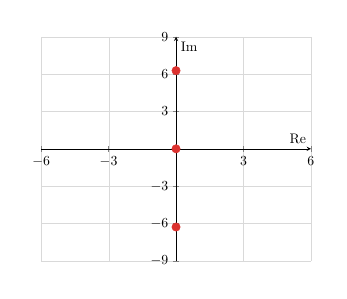
\begin{tikzpicture}[scale = 0.5]
      \begin{axis}[
          axis lines = center,
          xlabel = {Re},
          ylabel = {Im},
          xmin = -6, xmax = 6,
          ymin = -9, ymax = 9,
          grid = both,
          grid style = {line width=.1pt, draw=gray!30},
          xtick = {-9,-6,...,6,9},
          ytick = {-9,-6,...,6,9},
        ]
        % Plot discrete logarithm values (2kπi)
        \addplot[
          only marks,
          mark = *,
          mark size = 3pt,
          mark options = {custom_red}
        ] coordinates {
            (0, -6.28)
            (0, 0)
            (0, 6.28)
          };
      \end{axis}
    \end{tikzpicture}
  \end{minipage}



\end{examplebox}


\subsection{Complex Powers}
Recall the Logarithm Rule: $\log(a^b) = b\log(a)$. We want to define $z^\alpha$, in such a way that $\log(z^\alpha) = \alpha \log(z)$. That is the \textbf{Complex Power} is defined as:
$$z^{\alpha}  = e^{\alpha \log(z)} = e^{\alpha(\text{Log}(z) + 2k \pi i )} \quad \text{for} \, k \in \mathbb{Z}$$
So that we have:
\begin{align*}
  \log(z^\alpha) & = \log(e^{\alpha(\text{Log}(z) + 2k \pi i )}) \\
                 & = \alpha(\text{Log}(z) + 2k \pi i)            \\
                 & = \alpha \log(z)
\end{align*}
As example, consider $z = 1 + 0i$:
\begin{align*}
  1^{\alpha} & = e^{\alpha(Log(1) + 2k \pi i)} \\
             & = e^{2k \alpha \pi i}
\end{align*}
If $\alpha \in \mathbb{Z}$ $(1,2, 3, \dots)$
$$1^{\alpha} = \left(e^{2k \pi i}\right)^\alpha =  (\cos(2\pi k) + \sin(2\pi k))^\alpha = 1^\alpha = 1$$
If $\alpha = \frac{m}{n} \in \mathbb{Q}$, then $1^\alpha$ is the set of all $n$-th roots of unity:
$$1^{\alpha} = e^{\frac{2k\pi i m}{n}} = \cos\left(\frac{2\pi km}{n}\right) + i \sin\left(\frac{2\pi km}{n}\right) \cos\left(\frac{2\pi r}{n}\right) + i \sin\left(\frac{2\pi r}{n}\right)$$
If $\alpha = i$ then we see:
$$1^\alpha = 1^i = e^{2k\pi i \cdot i} = e^{-2k\pi}$$


\section{Geomtric Mappings and Transformations}
\subsection{Mappings:}
Recall we defined the principal branch as
$$\text{Log}(z) = \ln|z| + i \text{Arg}(z)$$
So, when we take the principal branch of the logarithm, we see that it maps to the complex number $w = u + iv$ where $u = \ln|z|$ and $v = \text{Arg}(z)$. \\
In essence. Log maps $\mathbb{C}$ to the horizontal strip:
$$\{w = u+iv: -\pi < v \leq \pi\}$$
\textbf{Diagram of the Logarithm Mapping:} \\
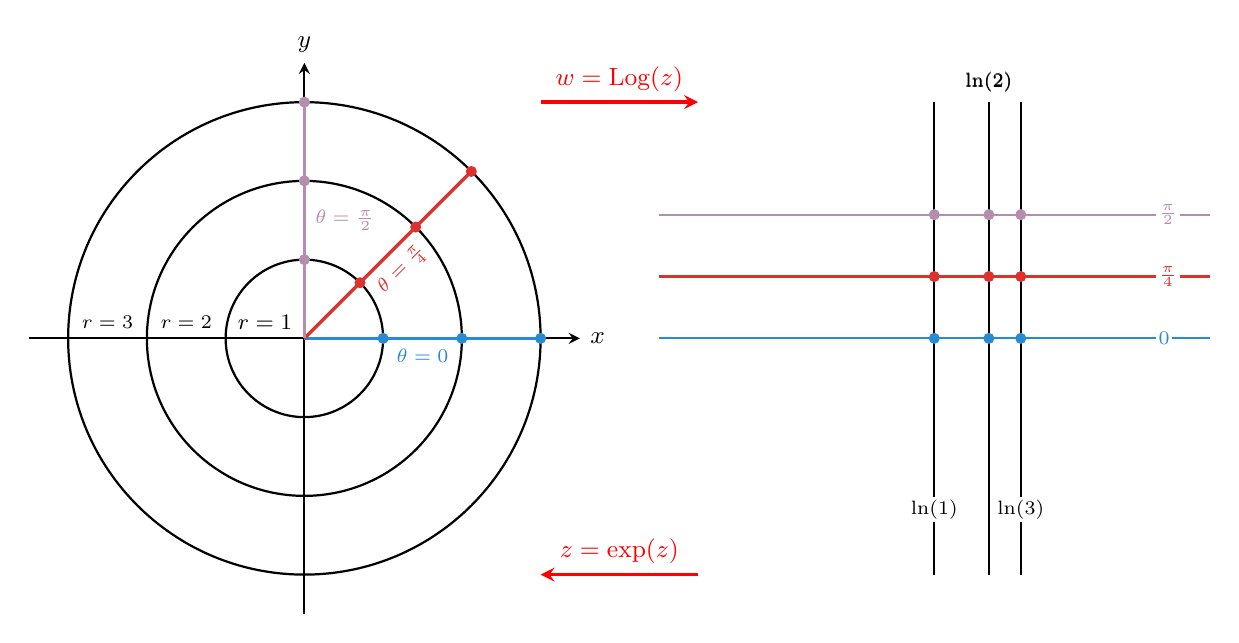
\begin{tikzpicture}[>=stealth, every node/.style={font=\small}, scale =1]

  \draw[->,thick] (-3.5,0) -- (3.5,0) node[right] {$x$};
  \draw[->,thick] (0,-3.5) -- (0,3.5) node[above] {$y$};
  \draw[black, thick] (0,0) circle (1);
  \node[black] at (-0.5,0.2) {\footnotesize$ r = 1$};

  \draw[black, thick] (0,0) circle (2);
  \node[black] at (-1.5,0.2) {\scriptsize$ r = 2$};
  \draw[black, thick] (0,0) circle (3);
  \node[black] at (-2.5, 0.2) {\scriptsize$ r = 3$};




  \draw[custom_blue, very thick] (0,0) -- (3,0) node[midway, below] {\scriptsize$\theta = 0$};
  \draw[custom_red, very thick] (0,0) -- (2.1213 ,2.1213)  node[midway, below, sloped] {\scriptsize$\theta = \frac{\pi}{4}$};
  \draw[custom_purple, very thick] (0,0) -- (0,3) node[midway, right] {\scriptsize$\theta = \frac{\pi}{2}$};

  \fill[custom_blue] (1,0) circle (2pt);
  \fill[custom_blue] (2,0) circle (2pt);
  \fill[custom_blue] (3,0) circle (2pt);

  \fill[custom_red] (0.707,0.707) circle (2pt);
  \fill[custom_red] (1.414,1.414) circle (2pt);
  \fill[custom_red] (2.12,2.12) circle (2pt);

  \fill[custom_purple] (0,1) circle (2pt);
  \fill[custom_purple] (0,2) circle (2pt);
  \fill[custom_purple] (0,3) circle (2pt);

  % Right coordinate system: (u,v) also with (0,0) centered.
  % Shift it horizontally so the two plots appear side by side.
  \begin{scope}[shift={(8,0)}]

    \pgfmathsetmacro{\lnone}{ln(1)}   % ln(1) = 0
    \pgfmathsetmacro{\lntwo}{ln(2)}   % ln(2) ≈ 0.693
    \pgfmathsetmacro{\lnthree}{ln(3)} % ln(3) ≈ 1.099

    % Draw vertical dashed lines at u = ln(1), ln(2), ln(3).
    \draw[dashed, black] (\lnone, -3) -- (\lnone, 3)
    node[pos=0.1667, anchor=north, fill=white, inner sep=1pt] {\scriptsize$\ln(1)$};
    \draw[dashed, black] (\lntwo, -3) -- (\lntwo, 3)
    node[above] {\scriptsize$\ln(2)$};
    \draw[dashed, black] (\lnthree, -3) -- (\lnthree, 3)
    node[pos=0.1667, anchor=north, fill=white, inner sep=1pt] {\scriptsize$\ln(3)$};

    \draw[thick, black] (\lnone, -3) -- (\lnone, 3)
    node[pos=0.1667, anchor=north, fill=white, inner sep=1pt] {\scriptsize$\ln(1)$};
    \draw[thick, black] (\lntwo, -3) -- (\lntwo, 3)
    node[above] {\scriptsize$\ln(2)$};
    \draw[thick, black] (\lnthree, -3) -- (\lnthree, 3)
    node[pos=0.1667, anchor=north, fill=white, inner sep=1pt] {\scriptsize$\ln(3)$};

    \draw[thick, custom_blue] (-3.5,0) -- (3.5,0)
    node[pos=0.9, anchor=west, fill=white, inner sep=1pt] {\scriptsize\(0\)};
    \draw[thick, custom_red] (-3.5,{pi/4}) -- (3.5,{pi/4})
    node[pos=0.9, anchor=west, fill=white, inner sep=1pt] {\scriptsize\(\frac{\pi}{4}\)};
    \draw[thick, custom_purple] (-3.5,{pi/2}) -- (3.5,{pi/2})
    node[pos=0.9, anchor=west, fill=white, inner sep=1pt] {\scriptsize\(\frac{\pi}{2}\)};

    \fill[custom_blue] (\lnone,0) circle (2pt);
    \fill[custom_blue] (\lntwo,0) circle (2pt);
    \fill[custom_blue] (\lnthree,0) circle (2pt);

    \fill[custom_red] (\lnone,{pi/4}) circle (2pt);
    \fill[custom_red] (\lntwo,{pi/4}) circle (2pt);
    \fill[custom_red] (\lnthree,{pi/4}) circle (2pt);

    \fill[custom_purple] (\lnone,{pi/2}) circle (2pt);
    \fill[custom_purple] (\lntwo,{pi/2}) circle (2pt);
    \fill[custom_purple] (\lnthree,{pi/2}) circle (2pt);

  \end{scope}




  \draw[->, very thick, red] (3,3) -- (5,3)
  node[midway, above,] {$ w= \text{Log}(z)$};

  \draw[<-, very thick, red] (3,-3) -- (5,-3)
  node[midway, above,] {$z= \text{exp}(z)$};

\end{tikzpicture}


\subsubsection{Example Mapping 1 :}
Let \( f(z) = z^3 \) \\
Using exponential rules and polar representation:
\begin{align*}
  z   & = |z|e^{i\theta}                                   \\
  z^3 & = \bigl(|z|e^{i\theta}\bigr)^3                     \\
      & = |z|^3 e^{i3\theta}                               \\
      & = |z|^3 \Bigl(\cos(3\theta) + i\sin(3\theta)\Bigr)
\end{align*}

Letting $z = 1 + 1i$, we see:
$\theta = \tan^{-1}\left(\frac{1}{1}\right) = 45^\circ = \frac{\pi}{4},$
and $|z| = \sqrt{1^2 + 1^2} = \sqrt{2}$.  Thus, we have: \\
\begin{minipage}{0.47\textwidth}
  \begin{align*}
    z^3 & = |z|^3\cdot \left[\cos(3\theta) + i\sin(3\theta)\right]                                            \\
        & = (\sqrt{2})^3\cdot \left[\cos\left(\frac{3\pi}{4}\right) + i\sin\left(\frac{3\pi}{4}\right)\right] \\
        & = -2\sqrt{2} + i 2\sqrt{2}
  \end{align*}
\end{minipage}\hfill
\begin{minipage}{0.47\textwidth}
  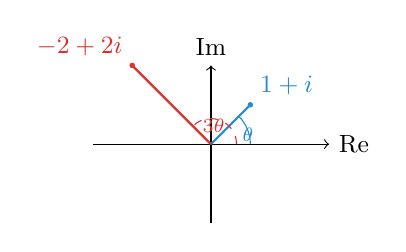
\begin{tikzpicture}[scale=0.5, every node/.style={font=\small}]

    % Draw the coordinate axes
    \draw[->] (-3,0) -- (3,0) node[right] {$\text{Re}$};
    \draw[->] (0,-2) -- (0,2) node[above] {$\text{Im}$};

    % Plot the complex number z = 1 + i (blue arrow)
    \draw[-, thick, custom_blue] (0,0) -- (1,1);
    \fill[custom_blue] (1,1) circle (2pt);
    \node[custom_blue, above right] at (1,1) {$1+i$};

    % Plot the complex number z^3 = -2 + 2i (red arrow)
    \draw[-, thick, custom_red] (0,0) -- (-2,2);
    \fill[custom_red] (-2,2) circle (2pt);
    \node[custom_red, above left] at (-2,2) {$-2+2i$};

    % Draw an arc for the angle of z (pi/4)
    \draw[custom_blue] (1,0) arc (0:45:1);
    \node[custom_blue, right] at (0.55,0.25) {\scriptsize$\theta$};

    % Draw an arc for the angle of z^3 (3pi/4)
    \draw[custom_red, dashed] (0.65,0) arc (0:135:0.65) node[below, right] {\scriptsize$3\theta$};

  \end{tikzpicture}
\end{minipage}\hfill
In essence, the mapping $f(z) = z^3$ rotates the complex number $z$ by $3\theta$ and scales it by $|z|^3$.
We can imagine this, for the complex numbers with $|z| = 1$, and $0 < \theta \leq \frac{\pi}{2}$, as an arc of radius $1$, from the angle $0 \to 90^\circ$, mapped to an arc of radius $8$, from the angles $0 \to 270^\circ$.


\subsubsection{Example Mapping 2}
We wish to find the image of the line \(x=1\) under
\[
  f(z)=\frac{1}{z}, \quad z=x+iy, \quad w=u+iv.
\]
For \(z=x+iy\) we have
\[
  w=\frac{1}{x+iy}=\frac{x-iy}{x^2+y^2}=\frac{x}{x^2+y^2}-i\frac{y}{x^2+y^2},
\]
so that
\[
  u=\frac{x}{x^2+y^2},\quad v=-\frac{y}{x^2+y^2}.
\]
Setting \(x=1\) yields
\[
  u=\frac{1}{1+y^2},\quad v=-\frac{y}{1+y^2}.
\]
Since
\[
  |w|^2=u^2+v^2=\frac{1}{1+y^2}=u,
\]
it follows that
\[
  u^2+v^2=u \quad\Longrightarrow\quad u^2-u+v^2=0.
\]
Completing the square in \(u\) by adding and subtracting \(\frac{1}{4}\):
\[
  u^2-u+\frac{1}{4}+v^2=\frac{1}{4} \quad\Longrightarrow\quad \left(u-\frac{1}{2}\right)^2+v^2=\frac{1}{4}.
\]
Thus, the image of \(x=1\) is the circle
\[
  \boxed{\left(u-\frac{1}{2}\right)^2+v^2=\frac{1}{4}},
\]
centered at \(\left(\frac{1}{2},0\right)\) with radius \(\frac{1}{2}\)
\begin{center}


  \begin{tikzpicture}[>=stealth, every node/.style={font=\small}, scale =2]

    \draw[->,thick] (-0.5,0) -- (1.5,0) node[right] {$x$};
    \draw[->,thick] (0,-1.5) -- (0,1.5) node[above] {$y$};

    \draw[-, thick, custom_blue] (1, -1.5) -- (1,1.5) node[pos=1, right] {$x=1$};


    % Right coordinate system: (u,v) also with (0,0) centered.
    % Shift it horizontally so the two plots appear side by side.
    \begin{scope}[shift={(5,0)}]
      \draw[->,thick] (-0.5,0) -- (1.5,0) node[right] {$u$};
      \draw[->,thick] (0,-1.5) -- (0,1.5) node[above] {$v$};
      \draw[custom_blue, thick] (0.5,0) circle (0.5);

      \draw[-, thick] (0.5, -0.1) -- (0.5,0.1) node[pos=-1] {\scriptsize$0.5$};


    \end{scope}




    \draw[->, very thick, red] (2,-1) -- (4,-1)
    node[midway, above,] {$ w= \frac{1}{z}$};


  \end{tikzpicture}

\end{center}
In general, $f(z) = \frac{1}{z}$ maps circle and lines to circles and lines, respectively.

\pagebreak

\subsection{Circle Preservation Theorem}
Consider the equation:
$$A(x^2 + y^2) + Bx + Cy + D = 0$$
We can we that if $A \neq 0$, then we can divide by $A$:
$$x^2 + y^2 + \frac{B}{A}x + \frac{C}{A}y + \frac{D}{A} = 0$$
Completing the square yields:
$$\left(x + \frac{B}{2A}\right)^2 + \left(y + \frac{C}{2A}\right)^2 = \left(\frac{B^2 + C^2 - 4AD}{4A^2}\right)$$
Thus, if $A\neq 0$, we have a circle with center (-B/2A, -C/2A) and radius $\sqrt{\frac{B^2 + C^2 - 4AD}{4A^2}}$. \\
If $A = 0$, then the equation represents a line:
$$Bx + Cy + D = 0$$
If $D = 0$, the circle or  line contains 0:
$$Bx + Cy + D \mid_{(0,0)} = D = 0$$
\textbf{Why is This Important?}\\[1mm]
Under the inversion $f(z) = \frac{1}{z}$ with $z = x+iy$ and $w = u+iv$, one can show that the general equation

$$A(x^2+y^2) + Bx + Cy + D = 0 \quad \underrightarrow{\text{maps to}} \quad D(u^2+v^2) + Bu - Cv + A = 0.$$

\noindent In this transformed equation:
\begin{itemize}
  \item If the original set does not contain the origin  image is a circle.
  \item If the original set does contain the origin then the equation becomes linear:

  \item If the original set is a line (with \(A=0\)), if it does not pass through the origin, its inversion is a circle that passes through the origin.
\end{itemize}
\noindent\textbf{Examples Illustrating the Inversion Effects} \\
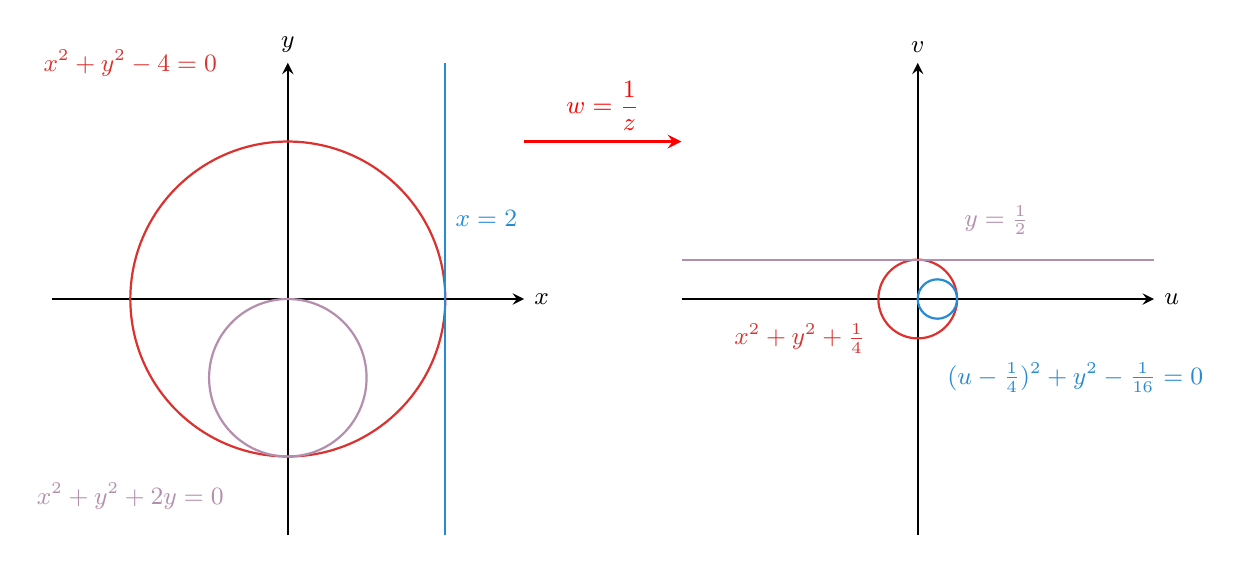
\begin{tikzpicture}[>=stealth, every node/.style={font=\small}, scale =1]

  \draw[->,thick] (-3,0) -- (3,0) node[right] {$x$};
  \draw[->,thick] (0,-3) -- (0,3) node[above] {$y$};
  \draw[custom_red, thick] (0,0) circle (2);
  \draw[custom_purple, thick] (0,-1) circle (1);
  \draw[custom_blue, thick, -] (2,-3) -- (2,3) node [pos=0.67, right] {$x=2$};

  \node[custom_red] at (-2,3) {$x^2 + y^2 -4 =0$};
  \node[custom_purple] at (-2,-2.5) {$x^2 + y^2 + 2y =0$};

  \begin{scope}[shift={(8,0)}]

    \draw[->,thick] (-3,0) -- (3,0) node[right] {$u$};
    \draw[->,thick] (0,-3) -- (0,3) node[above] {$v$};

    \draw[custom_red, thick] (0,0) circle (0.5);
    \draw[custom_purple, thick] (-3, 0.5) -- (3, 0.5);
    \draw[custom_blue, thick] (0.25,0) circle(0.25);

    \node[custom_purple] at (1,1) {$y = \frac{1}{2}$};
    \node[custom_blue] at (2,-1) {$(u-\frac{1}{4})^2 +y^2 - \frac{1}{16} = 0$};
    \node[custom_red] at (-1.5,-0.5) {$x^2 + y^2 + \frac{1}{4}$};
  \end{scope}





  \draw[->, very thick, red] (3,2) -- (5,2)
  node[midway, above,] {$ w= \dfrac{1}{z}$};


\end{tikzpicture}
\pagebreak
\subsection{Prelim to Riemann Sphere}
Our goal is to define the  \textbf{Riemann Sphere}, which is the complex plane $\mathbb{C}$, together with an extra point at infinity. In essence
The Riemann sphere is a way to "wrap  up" the entire complex plane into a compact, closed surface that is \textbf{homeomorphic} (toplogically equivalent) to the sphere $S^2$ and the connection between them is made via the \textbf{stereographic projection}.

\subsubsection{Euclidean Space and Compact Sets}
\textbf{Euclidean space}, denoted as \(\mathbb{R}^n\), is the collection of all points in \(n\)-dimensional space, where each point is described by \(n\) real numbers. In Euclidean spaces (such as the real line \(\mathbb{R}\) or the plane \(\mathbb{R}^2\)), a set is \textbf{compact} if it is both: \textbf{Closed} (contains all its limit points), and \textbf{Bounded} (contained within a finite region).

\begin{minipage}{0.47\textwidth}
  \begin{align*}
     & \textbf{Examples of Compact Sets:}                                                       \\
     & \text{The closed interval } [0,1] \subset \mathbb{R}^1,                                  \\
     & \text{A closed disk } \{(x,y) \in \mathbb{R}^2 : x^2 + y^2 \leq 1\} \subset \mathbb{R}^2
  \end{align*}
\end{minipage}\hfill
\begin{minipage}{0.47\textwidth}
  \begin{align*}
     & \textbf{Examples of Non-Compact Sets:}                                          \\
     & \text{The open interval } (0,1) \subset \mathbb{R}^1 \quad (\text{not closed}), \\
     & \text{The entire real line } \mathbb{R} \quad (\text{not bounded})
  \end{align*}
\end{minipage}

\subsubsection{Compactification of the Complex Plane}
The complex plane $\mathbb{C}$ is not compact - it streches out infinitely in all directions.
By adding a single point at infinity, we "close" the plane, turning it into a compact set.
This new space, is \textbf{homeomorphic} (a one-to-one mapping that is continuous
in both directions or toplogically equivalent) to  to the Riemann Sphere . We define the new space as:
$$\tilde{\mathbb{C}} = \mathbb{C} \cup \{\infty\}$$
\subsection{Riemann Sphere}
Define $\tilde{\mathbb{C}} = \mathbb{C} \cup \{\infty\}$. Then
$\tilde{\mathbb{C}} \xleftrightarrow{1:1} S^2 \{X = (x,y,z) : x^2 + y^2 + z^2 = 1 \}$
(\emph{homeomorphic}) via the sterographic projection, denoted $St$, defined as follows:\\[2ex]
\textbf{1. Projection from $S^2 \to \tilde{\mathbb{C}}$}: \\
For a point $(x, y,z ) \in S^2$, with $z \neq 1$ (the point is not the north pole) the projection is defined as:
\begin{gather}
  St(x, y, z) = \frac{1}{1-x_3}(x_1, x_2) \quad \text{for} \; z \neq 1 \notag \\
  \text{\emph{This takes a point on the sphere and maps it to a point in the complex plane.}} \notag
\end{gather}
\textbf{2. Projection from $\tilde{\mathbb{C}} \to S^2$}: \\
For a point $z \in \mathbb{C}$, the inverse projection is defined as:
\begin{gather}
  St^{-1}(z) = \frac{1}{|z|^2 + 1}\langle 2\text{Re}(z), 2\text{Im}(z), |z|^2 - 1 \rangle \notag  \\
  \text{\emph{This takes a complex number, $z$, written in terms of its real} $($Re$(z))$} \notag \\
  \text{\emph{and imaginary} $($Im$(z))$ \emph{parts, and maps it to the sphere}} \notag
\end{gather}
\textbf{3. Mapping the North Pole}:
\\The projection leaves out the north pole from projection onto $\mathbb{C}$
\begin{gather}
  St(N)= \infty \quad \text{and} \quad St^{-1}(\infty) = N \notag \quad \text{where}\; N = \langle 0,0,1\rangle\\
  \text{\emph{The north pole is mapped to the point at infinity, and vice versa.}} \notag
\end{gather}

\pagebreak

\section{Complex Analysis}
\subsection{Mobius Transforms}
\textbf{Recall:} The complex plane $\mathbb{C}$ can be throught as points $(x,y) \in \mathbb{R}^2$, but we usually label a point as $z = x+iy$.
We can extend $\mathbb{C}$ by adding a point at infinity, the resulting set is called the \textbf{Riemann Sphere} $\tilde{\mathbb{C}}$.
Visually, we can imaigine wrapping the complex plane onto the surface of a sphere, where $\infty$ is the north pole of the sphere. \\[2ex]
\noindent Now, letting $a,b,c,d$ be complex numbers (i.e. $ a = x_a + iy_a$), we define a Mobius Transform as a function $T:\tilde{\mathbb{C}} \to \tilde{\mathbb{C}}:$
$$T(z) = \frac{az + b}{cz +d}$$
where $ad -bc \neq 0$ (that is the determinant $\neq$ 0 $\rightarrow$ matrix is invertible). \\
These functions occur on the Riemann Sphere, because we need to define that happens when $cz + d = 0$ and when $z = \infty$:

$$\text{If} \;c \neq 0: \quad T(\infty) = \frac{a}{c} \quad \text{and} \quad T\left(-\frac{d}{c}\right) = \infty$$
$$\text{If} \;c = 0: \quad T(z) = \frac{az + b}{d}\quad \text{and} \quad T(\infty) = \infty$$

\noindent Mobius transforms can be  uniquely determined by its action on three distinct points. For example, we'll find a mobius transform that maps three points $\{z_1, z_2, z_3\}$ to $\{1,0,\infty\}$ \\[2ex]
1. We want $T(z_2) = 0 : az_2 + b = 0 \Rightarrow b= -az_2$ , then $T(z)$ becomes:
$$T(z) = \frac{az + b}{cz + d} = \frac{az -az_2}{cz+d} = \frac{a(z-z_2)}{cz + d}$$
2. We want $T(z_3) = \infty : cz_3 + d = 0 \Rightarrow d = -cz_3$, then $T(z)$ becomes:
$$T(z) = \frac{a(z - z_2)}{c(z - z_3)}$$
3. We want $T(z_1) = 1$, then $T(z_1)$ becomes:
$$T(z_1) = \frac{a(z_1 - z_2)}{c(z_1 - z_3)} = 1 \Rightarrow \frac{a}{c} = \frac{z_1 - z_3}{z_1 - z_2}$$
Finally, we see that $T(z)$ is:
$$T(z) = \frac{z_1 - z_3}{z_1 - z_2}\cdot \frac{z - z_2}{z - z_3} $$
We can now solve problems, such as : Find the Mobius Transform that maps the 3 points $z_1 = -i, z_2 = -1, z_3 = 1$ to $1,0,\infty$
$$T(z) = \frac{-1 -1}{i + 1} \cdot \frac{z + 1}{z-1} = (-i)\frac{z+1}{z-1} = \frac{-iz -i}{z-1}$$

\pagebreak

\subsubsection{Matrix Representation of Mobius Transforms}
We associate a $2 \times 2$ matrix $M$ to a Mobius Transform $T(z)$:
$$T(z) = \frac{az + b}{cz + d} \longleftrightarrow M  = \begin{bmatrix}a & b \\c & d\end{bmatrix}$$
\indent \emph{Note that:} $kM \longleftrightarrow T(z)$ for any $k \in \mathbb{C}, k \neq 0$. \\[2ex]
We can also define the \textbf{inverse map} $T^{-1}$ as the Mobius transform:
$$T^{-1} \longleftrightarrow \begin{bmatrix}d & -b \\ -c & a\end{bmatrix}$$
We can also define the \textbf{composition} of two Mobius Transforms, if $T_1(z) = \frac{az + b}{cz + d}$ with matrix $M$ and $T_2(z) = \frac{ez + f}{gz + g}$ with matrix $M_2$, then:
$$
  T \circ T_2 \longleftrightarrow
  \begin{bmatrix}
    a & b \\ c & d
  \end{bmatrix}
  \cdot
  \begin{bmatrix}
    e & f \\ g & h
  \end{bmatrix}
  =
  \begin{bmatrix}
    ae + bg & af + bh \\ ce + dg & cf + dh
  \end{bmatrix}
$$
Putting it all together, we can map any three points to any other three point:
\begin{theorembox}[Three-Point Theorem for Möbius Transformations]
  \footnotesize If $T \longleftrightarrow M : (z_1, z_2, z_3) \mapsto (1,0,\infty)$ and if $T_2 \longleftrightarrow M_2: (z'_1, z'_2, z'_3) \mapsto (1,0,\infty)$ then:
  $$T^{-1} \circ T_2 \longleftrightarrow M^{-1} \cdot: (z_1, z_2, z_3) f\mapsto (z'_1, z'_2, z'3) $$
  This can be visualized like so:
  \begin{center}
    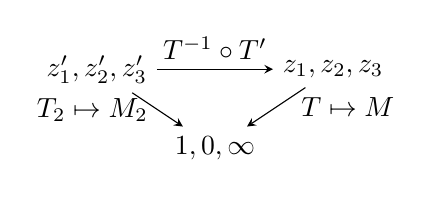
\begin{tikzpicture}[>=stealth, auto]
      \node (A) at (0,1) {$z'_1, z'_2, z'_3$};
      \node (B) at (3, 1) {$z_1, z_2, z_3$};
      \node (C) at (1.5,0) {$1, 0, \infty$};

      \draw[->] (A) -- (B) node[above, midway] {$T^{-1} \circ T'$};
      \draw[->] (A) -- (C) node[left, midway] {$T_2 \mapsto M_2$};
      \draw[->] (B) -- (C) node[right, midway] {$\;\;T \mapsto M$};
    \end{tikzpicture}
  \end{center}
  Note that, $M, M_2$ and $T^{-1}\circ T_2$ have matrices: Three-Point Theorem for Mobius Transformations
  $$M = \begin{bmatrix} a&b \\ c &d \end{bmatrix}, \quad M_2 = \begin{bmatrix} e&f \\ g &g \end{bmatrix},
    \quad T^{-1} \circ T_2 =  \begin{bmatrix} d&-b \\ -c &a \end{bmatrix} \cdot \begin{bmatrix}e & f \\ g & h\end{bmatrix}$$
\end{theorembox}

\begin{examplebox}{Find a Mobius transformation, $T:  (0,-i,-1) \mapsto (i, 1, 0)$}{}
  \footnotesize If we can find a map $T_1 : (0, -i, 1) \mapsto (1, 0, \infty)$ and a map \\
  $T_2 : (1, -i, -1) \mapsto (i, 1, 0)$. Then, by the Theorem above, we can find a $T$ such that: $T:(0, -i, -1) \mapsto (i, 1,0)$
  Recall, we define a general transform $T$, that takes 3 points $(z_1, z_2, z_3) \mapsto (1, 0, \infty)$
  $$T(z) = \frac{z_1 - z_3}{z_1 - z_2} \cdot \frac{z - z_2}{z - z_3} $$
  \noindent
  \scriptsize\begin{minipage}{0.45\textwidth}
    $T_1$ becomes:
    \begin{align*}
      T_1(z) & = \frac{0 +1}{0+i} \cdot \frac{z+i}{z+1}                \\
             & = \frac{1}{i}\cdot \frac{z+i}{z+1}                      \\
             & = \frac{z+1}{iz + i}                                    \\
             & \Rightarrow \begin{bmatrix}1 & i \\ i & i \end{bmatrix}
    \end{align*}
  \end{minipage}
  \begin{minipage}{0.45\textwidth}
    $T_2$ becomes:
    \begin{align*}
      T_2(z) & = \frac{i-0}{i-1} \cdot \frac{z-1}{z-0}                    \\
             & = \frac{i}{i-1} \cdot \frac{z-1}{z}                        \\
             & = \frac{iz - i}{(i-1)z }                                   \\
             & \Rightarrow \begin{bmatrix}i & -i \\ i-1 & 1 \end{bmatrix}
    \end{align*}
  \end{minipage}
  \hfill \\[2ex]
  Thus, $T$ is:
  $$T =T^{-1}_2 \circ T_1 \leftrightarrow \begin{bmatrix}1 & i \\ i & i\end{bmatrix} \cdot \begin{bmatrix} i & -i \\ i-1 & 0 \end{bmatrix}^{-1}$$
  \scriptsize$$
    = \begin{bmatrix}1 & i \\ i & i\end{bmatrix} \cdot \begin{bmatrix}0 & i \\ 1 & i-1\end{bmatrix}
    = \begin{bmatrix}1 & i \\ i & i\end{bmatrix} \cdot \begin{bmatrix}i & -i \\ i-1 & 1\end{bmatrix}
    = \begin{bmatrix} 0(1) + (i)(i) & (0)(i) + (i)(i) \\ (1-i)(1)+ (i)(i) & (1-i)(i) + (i)(i)\end{bmatrix}
    = \begin{bmatrix} i^2 & i^2 \\ -i & i\end{bmatrix}
  $$
  \normalsize$$T(z)  = -\begin{bmatrix}1 & 1 \\ i & -i \end{bmatrix}\longleftrightarrow = -i \frac{z+1}{z-1}$$

\end{examplebox}

\pagebreak

\subsection{Complex Differentiation}
First we must define what is meant for a set to be \textbf{open} in the complex plane.
\subsubsection{Open Sets in the Complex Plane}
\begin{definitionbox}{}{}
  We say a subset $\mathbb{U} \subseteq \mathbb{C}$ is \textbf{open} if $\forall\;  z_0 \in \mathbb{U} \quad \exists \; \varepsilon   > 0$
  such that the open disc centered at $z_0$ of radius $\varepsilon$ is contained in $\mathbb{U}$:
  $$D_{\varepsilon} (z_0) = \{z \in \mathbb{C} \mid |z-z_0| < \varepsilon\}$$ \\
  \centering
  \begin{tikzpicture}
    \draw[dashed] (0,0) rectangle (4,2);
    \draw[dotted] (1.5,1) circle (0.5);
    \filldraw (1.5,1) circle (0.05) node[below] {$z_0$};
    \draw[->] (1.5,1) -- (2,1) node[midway, above] {$\varepsilon$};
    \node at (4.2,1.8) {$\mathbb{U}$};
  \end{tikzpicture}
\end{definitionbox}
\noindent In essence, a set $\mathbb{U}$ in the complex plane is defined as open if for every point $z_0$ in $\mathbb{U}$,
you can draw a small circle around $z_0$ that fits entirely within $\mathbb{U}$. This radius of this circle is $\varepsilon$. The
radius can be very small but must be positive.
\subsubsection{Differentiation}
\begin{definitionbox}{}{}
  Let $\mathbb{U} \subseteq \mathbb{C}$ be open, let $f: \mathbb{U} \to \mathbb{C}$ be a function and let $z_0 = x_0 + iy_0 \in \mathbb{U}$.
  $$f'(z_0) = \lim_{h \to 0} \frac{f(z_0 + h) - f(z_0)}{h}$$
  If the limit exists, independant of the direction of approach we say $f$ is \textbf{holomorphic} (or complex differentiable / complex analytic) \textbf{at} $z_0$.
  We also call $f'(z_0)$ the derivative of $f$ at $z_0$. \\
  Similarly, if $f$ is holomorphic $\forall \; z \in \mathbb{U}$ we say $f$ is holomorphic \textbf{on} $\mathbb{U}$.
\end{definitionbox}


\subsubsection{Cauchy-Riemann Equations}
\begin{theorembox}[: Cauchy-Riemann Equations]
  If $f:\mathbb{U} \to \mathbb{C}$ is holomorphic on $\mathbb{U} \subseteq \mathbb{C}$, then for $z = x + iy$ and $f(z) = u(x,y) + iv(x,y)$, we have:
  $$\pdiff{u}{x} = \pdiff{v}{y} \quad  \text{and} \quad \pdiff{u}{y} = - \pdiff{v}{x}$$
\end{theorembox}

\pagebreak

\subsubsection{Jacobian Matrix}
The Jacobian matrix represents how a function transforms small regions in space. For a function that maps $n$ dimensional space $\to$ $m$ dimensional space,
the Jacobian contains all partial derivatives arranged in an $m \times n$ matrix.
For example, $f$ as a map $f: \mathbb{R}^2 \to \mathbb{R}^2$, has the Jacobian matrix:
$
  Df =
  \begin{pmatrix}
    u_x & u_y \\
    v_x & v_y
  \end{pmatrix}$
Which for $(x_0, y_0) \in \mathbb{R}^2$ gives an $2 \times 2$ matrix:
$$Df(x_0, y_0) =
  \begin{pmatrix}
    u_x(x_0, y_0) & u_y(x_0, y_0) \\
    v_x(x_0, y_0) & v_y(x_0, y_0)
  \end{pmatrix}
  :
  \mathbb{R}^2 \to \mathbb{R}^2
$$
Now, $f$ statisfies the Cauchy-Riemann equations:
$$
  \begin{pmatrix}
    u_x & u_y \\
    v_x & v_y
  \end{pmatrix}
  \begin{pmatrix}
    0 & -1 \\
    1 & 0
  \end{pmatrix}
  =
  \begin{pmatrix}
    0 & -1 \\
    1 & 0
  \end{pmatrix}
  \begin{pmatrix}
    u_x & u_y \\
    v_x & v_y
  \end{pmatrix}
$$
Where, the matrix $\begin{psmallmatrix} 0 & -1 \\ 1 & 0 \end{psmallmatrix}$ is the rotation matrix for $\pi / 2$ ($90^{\circ}$). Meaning that the map $Df$ is $\mathbb{C}$-linear, that is it preserves addition and complex scalar multiplication:
$$f(x + y) = f(x) + f(y)$$
$$f(\alpha x) = \alpha f(x), \quad \forall \alpha \in \mathbb{C}$$

\subsection{Complex Integration}


\end{document}